\section{Exercise 1}

For this first exercise we had to write our own Poisson probability distribution function and random number generator. 

The functions that I wrote for this exercise can be found in: 
\lstinputlistin{NR_a1_1_utils.py}

The commands used to retrieve the desired results are given by:
\lstinputlistin{NR_a1_1_mail.py}

\begin{figure}[h!]
  \centering
  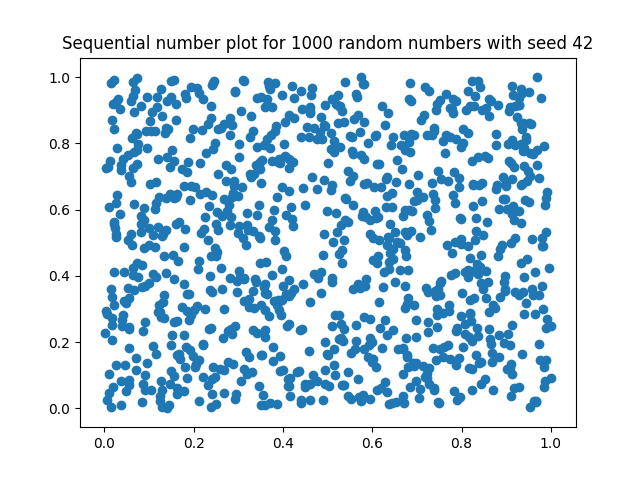
\includegraphics[width=0.9\linewidth]{./plots/1_b_1.png}
  \caption{In this figure we can see that it appears that the random number generator is producing numbers without a certain preference.}
  \label{fig:fig1.1}
\end{figure}

\begin{figure}[h!]
  \centering
  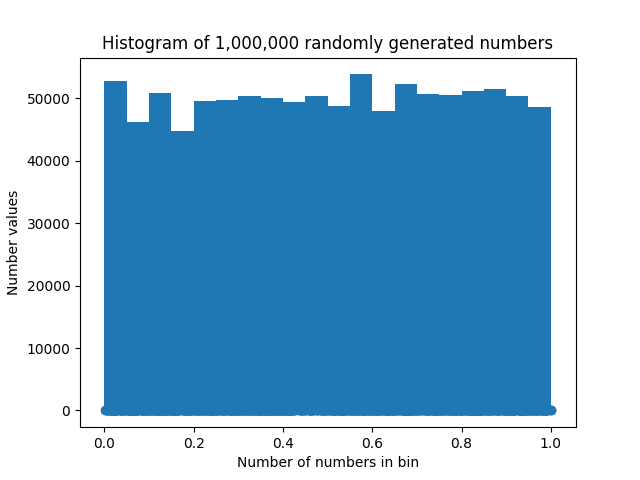
\includegraphics[width=0.9\linewidth]{./plots/1_b_2.png}
  \caption{This histogram places the random number generator under a sharper knife, allowing us to see that there are some fluctuations between the bins. Overal it appears to be quite unbiased.}
  \label{fig:fig1.2}
\end{figure}
